	\section{Цель работы}
		Разработать экспертную систему с использованием среды GURU.
		
	\section{Предметная область}
		Целевая ЭС выполняет функцию оценки платформ для социальной торговли. Социальная торговля -- онлайн-трейдинг на финансовых рынках в рамках социальной платформы, внутри которой трейдеры взаимодействуют друг с другом.
		
		На рисунке \ref{tree} изображено дерево целей экспертной системы. Дугами отмечены вершины И, отсутствием дуг ИЛИ.
		
		\begin{figure}[ht] 
			\center
			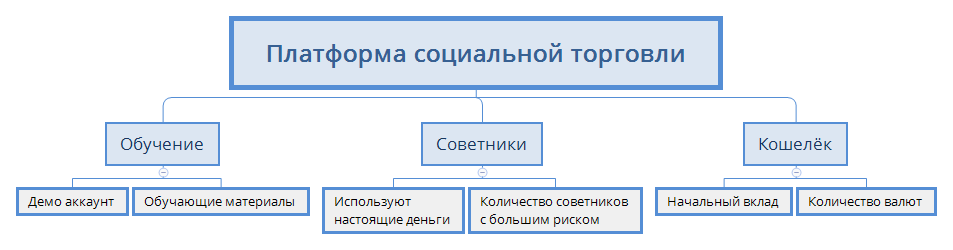
\includegraphics [width=\textwidth] {social-trading}
			\caption{Дерево целей} 
			\label{tree}
		\end{figure}
		\FloatBarrier
		
	\section{Описание ЭС}
	
	На основе дерева целей описаны переменные и правила, представленные в листинге.
	
	Системная переменная $ E.CFVA $, которая определяет формулу объединения факторов уверенности левой и правой частей правила имеет значение <<pp>>, т.е. фактор уверенности для операции <<И>> вычисляется по формуле $(a * b) / 100$, а для правила <<ИЛИ>> - по формуле 	$a + b - (a * b) / 100$
	
	Системная переменная $E.TRAC = <n>$ определяет режим работы системы – без трассировки.
	
	С помощью переменной $E.RIGR$ определяется режим проверки конфликтующих правил для достижения результата с заданной степенью точности. $E.RIGR = <с>$ – все возможные правила (полный перебор).
	
	Режим оценки $E.TRYP = <s>$ - проверка неизвестных переменных, пока значение какой-либо из них не будет получено.
	 
	$E.LNUM = 3$ -  длина числового значения для округления.
	
	$E.DECI = 0$ - число значащих цифр после запятой.
	
		
	\section{Листинг}
	
	\lstinputlisting[caption={Листинг программы}]{listings/st.rss}
	
	\newpage
	\section{Примеры выполнения}
		На рисунке \ref{img:good} представлен пример хорошей платформы. Расчёт, в соответствии с формулами в листинге, где $\vee$ - операция <<И>>:
		
		
		\begin{multline}
			\frac{cfDEMO \vee \frac{3 * cfMATERIALS}{4}}{2} 
			\vee \frac{\frac{cfMINSTART}{2} \vee cfCURRENCIES}{2}\vee \\
			\vee\frac{(\frac{2*cfREALMONEY}{3} \vee cfRSKY )*3}{4} =
			\frac{90 \vee \frac{3 * 60}{4}}{2} \vee
			\frac{\frac{70}{2} \vee 75}{2}\vee 
			\frac{(\frac{2*100}{3} \vee 79 )*3}{4} =\\
			=47 \vee 30 \vee 68 = 63 \vee 68
			= 87\\
		\end{multline}

		
		\begin{figure}[ht] 
			\center
			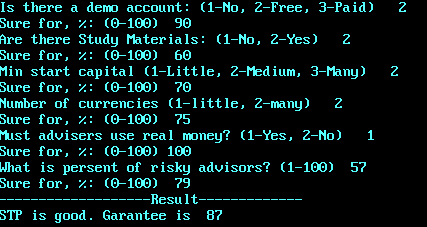
\includegraphics [width=\textwidth] {success}
			\caption{Пример хорошей платформы} 
			\label{img:good}
		\end{figure}
		\FloatBarrier
		
		\begin{multline}
			 \frac{ \frac{cfDEMO*3}{4} \vee \frac{3 * (100-cfMATERIALS)}{4}}{2} \vee\\
			\vee \frac{\frac{(100-cfMINSTART)}{4} \vee (100-cfCURRENCIES)}{2}\vee \\
			\vee\frac{(\frac{2*(100-cfREALMONEY)}{3} \vee cfRSKY )*3}{4} =\\
			 \frac{ \frac{70*3}{4} \vee \frac{3 * (100-70)}{4}}{2} \vee
			\frac{\frac{(100-70)}{4} \vee (100-70)}{2}\vee 
			\frac{(\frac{2*(100-70)}{3} \vee 70 )*3}{4} = 61\\
		\end{multline}
		
		
		\begin{figure}[ht] 
			\center
			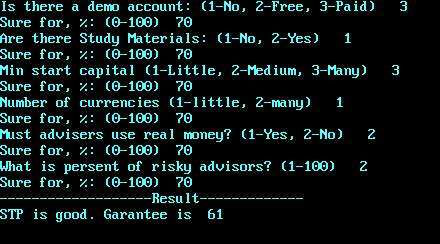
\includegraphics [width=\textwidth] {middle}
			\caption{Пример средней платформы} 
		\end{figure}
		\FloatBarrier
		
		\begin{multline}
			 \frac{ (100-cfDEMO )\vee \frac{3 * (100-cfMATERIALS)}{4}}{2} \vee\\
			\vee \frac{\frac{(100-cfMINSTART)}{4} \vee (100 - cfCURRENCIES)}{2}\vee \\
			\vee\frac{(\frac{2*(100-cfREALMONEY)}{3} \vee (100-cfRSKY))*3}{4} =\\
			 \frac{ (100-80 )\vee \frac{3 * (100-60)}{4}}{2} \vee
			\frac{\frac{(100-90)}{4} \vee (100 - 40)}{2}\vee \\
			\vee\frac{(\frac{2*(100-90)}{3} \vee (100-10))*3}{4}  = 74\\
		\end{multline}
		
		
		\begin{figure}[ht] 
			\center
			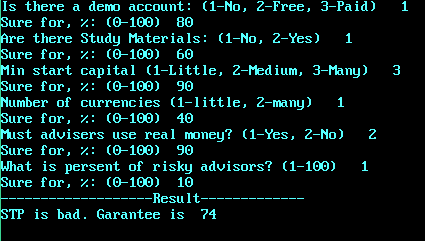
\includegraphics [width=\textwidth] {failure}
			\caption{Пример плохой платформы} 
		\end{figure}
		\FloatBarrier
	
	\section{Вывод}
		В результате данной работы была спроектирована разработана ЭС, которая позволяет дать экспертную оценку платформам социальной торговли по введенным параметрам. Изучена программа GURU.